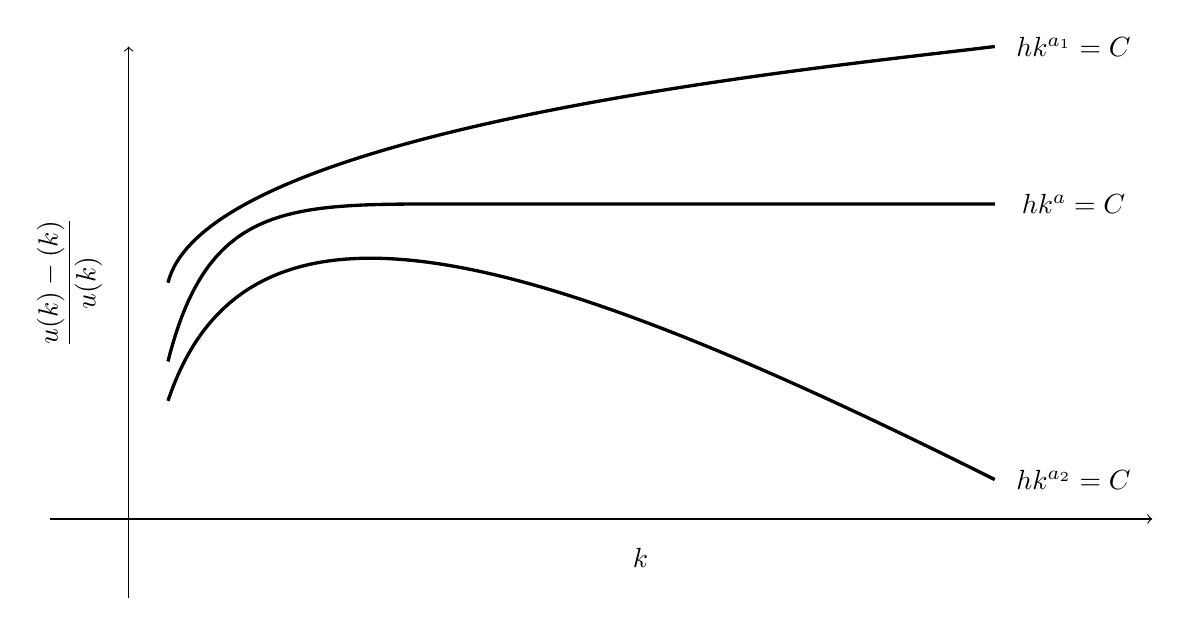
\begin{tikzpicture}
  
% axes
  
  \draw[->] (-1.0,0.0) -- (13.0,0.0);
  \draw[->] (0.0,-1.0) -- (0.0,6.0);

  \draw (6.5,-0.5) node {$k$};

  \draw (-0.75,3.0) node {\rotatebox{90}{$\displaystyle \frac{\NHokD{u(k)-\uh(k)}}{\NHokD{u(k)}}$}};
  % Found out about rotatebox from https://tex.stackexchange.com/a/45852

  

  % Good graph
  \draw[very thick] (0.5,2.0) .. controls (1.0,4.0) and (2.0,4.0) .. (4.0,4.0) -- (11.0,4.0);

  \draw (12.0,4.0) node {$hk^{a}=C$};

  % Bad graph
  \draw[very thick] (0.5,3.0) .. controls (1.0,5.0) and (9.0,5.75) .. (11.0,6.0);

    \draw (12.0,6.0) node {$hk^{a_{1}}=C$};

  % Overgood graph
    \draw[very thick] (0.5,1.5) .. controls (1.5,4.5) and (5.0,3.5) .. (11.0,0.5);

        \draw (12.0,0.5) node {$hk^{a_{2}}=C$};
  
  \end{tikzpicture}
